% Source : http://tex.stackexchange.com/questions/44673/sieve-of-eratosthenes-in-tikz

\documentclass{article}   
\usepackage{tikz}    
\makeatletter
\newcommand\coordsphere[1]{% where we put the number
     \pgfmathparse{mod(#1,10)}   
    \ifnum 0=\pgfmathresult      \global\def\yc{10}  \else  \global\let\yc\pgfmathresult \fi     
    \pgfmathparse{(#1-\yc)/10)}  \global\let\xc\pgfmathresult 
    \def\position{\yc-1,\xc+1} 
    }%   
\newcommand\testcolorednode[3]{%
   \pgfutil@ifundefined{pgf@sh@ns@#1}{#2}{#3}}% is named node ? 
\makeatother

\begin{document}
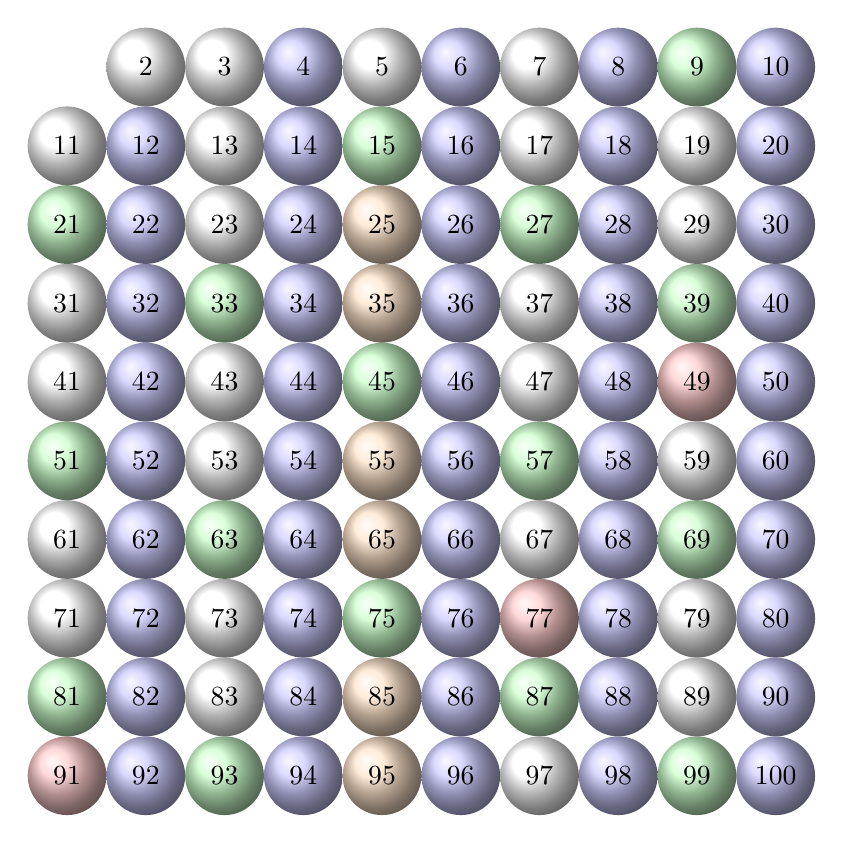
\begin{tikzpicture}[y=-1cm,every node/.style={minimum size= 1cm,circle}] 
 \foreach \p/\c in {2/blue,3/green,5/orange,7/red} {%  test only 4 prime numbers, we need 4 colors
    \pgfmathtruncatemacro{\start}{\p+1}
    \foreach \nb in {\start,...,100} {%
       \coordsphere{\nb}%                          where ?? find the position 
       \pgfmathifthenelse{mod(\nb,\p)==0}{0}{1}%   test if \nb is multiple of \p 
       \ifnum \pgfmathresult=0      
              \testcolorednode{\nb}% test if \nb is the name of a node if no we write the number
                                   % else we draw a sphere with and we give a name to the node
               {\node[ball color=\c!20](\nb) at (\position) {\nb};}
               {}     
       \fi}}  
  \foreach \nb in {2,...,100} {% Now we test all the numbers, if a number is not inside a node with       
                              % a name then we draw the sphere in white. The number is  prime.
      \coordsphere{\nb}% where ?? find the position
      \testcolorednode{\nb}{\node[ball color=white](\nb) at (\position) {\nb};}{}
  }    
\end{tikzpicture} 
\end{document}
